\documentclass[12pt]{article}

\usepackage{fullpage}
\usepackage{multicol,multirow}
\usepackage{tabularx}
\usepackage{ulem}
\usepackage[utf8]{inputenc}
\usepackage[russian]{babel}
\usepackage{float}
\usepackage{graphicx}


% Оригиналный шаблон: http://k806.ru/dalabs/da-report-template-2012.tex

\begin{document}

\section*{Лабораторная работа №\,2 по курсу дискрeтного анализа: cбалансированные деревья}

Выполнил студент группы 08-207 МАИ \textit{Дружинин Данила}.

\subsection*{Условие}

 
\begin{enumerate}
\item В данной лабораторной работе требовалось создать программную библиотеку, реализующую указанную структуру данных, на основе которой разработать программу-словарь. Словарь должен хранить пары вида «ключ--значение», где ключом является регистронезависимое слово, состоящее из букв английского алфавита длиной не более 256 символов, а значением --- целое беззнаковое число из диапазона от 0 до $2^{64} - 1$. Программа должна обрабатывать входные данные построчно до конца файла и поддерживать основные операции словаря: добавление нового слова, удаление существующего слова и поиск слова с выводом связанного с ним значения. 
\item Задача 1. 1 AVL-дерево
\end{enumerate}

\subsection*{Метод решения}

В данной работе реализован словарь на основе сбалансированного двоичного дерева поиска (AVL-дерева). Структура данных хранит пары «ключ--значение», где ключом является строка фиксированной длины, а значением --- число типа \texttt{uint64\_t}.

Каждый узел дерева содержит:
\begin{itemize}
	\item строковый ключ;
	\item числовое значение;
	\item высоту узла;
	\item указатели на левое и правое поддеревья.
\end{itemize}

Дерево удовлетворяет свойству бинарного дерева поиска: для каждого узла все ключи в левом поддереве меньше текущего, а в правом --- больше.

Балансировка дерева осуществляется с использованием высот поддеревьев. Для каждого узла вычисляется разность высот левого и правого поддеревьев. Если эта разность выходит за пределы допустимого значения, выполняются повороты дерева (левый или правый, а также их комбинации) для восстановления баланса.

Основные операции реализованы рекурсивно.

\textbf{Поиск} выполняется аналогично поиску в бинарном дереве поиска: на каждом шаге производится сравнение строк, и переход осуществляется в левое или правое поддерево.

\textbf{Вставка} производится следующим образом. Если текущий узел отсутствует, создаётся новый узел. В противном случае выполняется сравнение ключей:
\begin{itemize}
	\item если ключ уже существует, вставка не производится;
	\item если ключ меньше текущего, вставка выполняется в левое поддерево;
	\item если больше --- в правое.
\end{itemize}
После вставки пересчитывается высота узла и при необходимости выполняется балансировка дерева с помощью поворотов.

\textbf{Удаление} также реализовано рекурсивно. При нахождении узла:
\begin{itemize}
	\item если у узла отсутствует один из потомков, он заменяется другим поддеревом;
	\item если оба потомка существуют, выбирается узел с минимальным ключом в правом поддереве, после чего выполняется замена и рекурсивное удаление.
\end{itemize}
После удаления производится обновление высот и балансировка дерева.

Для обеспечения регистронезависимости ключей все входные строки приводятся к нижнему регистру. Для работы со строками используются собственные функции сравнения и копирования.

Обработка входных данных осуществляется построчно. В зависимости от команды вызываются операции вставки, удаления или поиска.

Реализованная структура обеспечивает выполнение операций вставки, поиска и удаления за логарифмическое время.

\subsection*{Описание программы}

Программа реализована в одном исходном файле на языке C++ и представляет собой консольное приложение. Для работы используются стандартные библиотеки языка для ввода-вывода, работы с типами данных и файлами.

\vspace{1\baselineskip}
\textbf{Основная структура данных}
\vspace{1\baselineskip}

Ключевым элементом программы является структура узла дерева:

\begin{itemize}
	\item \texttt{TNode} --- структура, описывающая узел AVL-дерева. Она содержит:
	\begin{itemize}
		\item массив символов фиксированного размера для хранения ключа;
		\item значение типа \texttt{uint64\_t};
		\item поле \texttt{Height}, хранящее высоту поддерева;
		\item указатели на левое и правое поддеревья (\texttt{Left}, \texttt{Right}).
	\end{itemize}
\end{itemize}

\textbf{Класс словаря}

Для работы с деревом реализован класс \texttt{TAvlDictionary}, который содержит указатель на корень дерева (\texttt{Root}) и предоставляет интерфейс для выполнения операций со словарём:

\begin{itemize}
	\item \texttt{Insert} --- добавление нового элемента. Возвращает признак успешности вставки;
	\item \texttt{Find} --- поиск элемента по ключу с возвратом соответствующего значения;
	\item \texttt{Erase} --- удаление элемента по ключу;
	\item \texttt{Clear} --- удаление всех узлов дерева;
	\item \texttt{Save} --- сохранение текущего состояния словаря в бинарный файл;
	\item \texttt{Load} --- загрузка словаря из файла с заменой текущего состояния.
\end{itemize}

\textbf{Реализация дерева}

Работа дерева обеспечивается набором вспомогательных функций:

\begin{itemize}
	\item \texttt{InsertNode} --- рекурсивная вставка узла с последующей балансировкой;
	\item \texttt{FindNode} --- поиск узла по ключу;
	\item \texttt{EraseNode} --- удаление узла с последующей балансировкой;
	\item \texttt{FindMin} --- поиск узла с минимальным ключом в поддереве;
	\item \texttt{RemoveMin} --- удаление узла с минимальным ключом;
	\item \texttt{ClearTree} --- рекурсивное удаление всех узлов дерева.
\end{itemize}

\textbf{Балансировка дерева}

Для поддержания сбалансированности используются следующие функции:

\begin{itemize}
	\item \texttt{GetHeight} --- получение высоты узла;
	\item \texttt{FixHeight} --- пересчёт высоты узла на основе высот поддеревьев;
	\item \texttt{BalanceFactor} --- вычисление разности высот левого и правого поддеревьев;
	\item \texttt{RotateLeft}, \texttt{RotateRight} --- повороты дерева;
	\item \texttt{Balance} --- приведение узла к сбалансированному состоянию.
\end{itemize}

\textbf{Работа со строками}

Поскольку стандартные строковые типы не используются, реализованы собственные функции:

\begin{itemize}
	\item \texttt{StrLen} --- вычисление длины строки;
	\item \texttt{StrCopy} --- копирование строки;
	\item \texttt{StrCompare} --- лексикографическое сравнение строк;
	\item \texttt{ToLowerWord} --- приведение строки к нижнему регистру.
\end{itemize}

\textbf{Работа с вводом данных}

Для разбора входных данных используются функции:

\begin{itemize}
	\item \texttt{ReadWord} --- чтение слова из строки;
	\item \texttt{ReadUInt64} --- чтение числового значения;
	\item \texttt{SkipSpaces} --- пропуск пробельных символов;
	\item \texttt{RemoveNewline} --- удаление символов конца строки.
\end{itemize}

\textbf{Сохранение и загрузка}

Для работы с файлами реализованы функции:

\begin{itemize}
	\item \texttt{SaveNodes} --- последовательная запись узлов дерева в файл;
	\item \texttt{LoadNodes} --- чтение узлов из файла и восстановление дерева;
	\item \texttt{CountNodes} --- подсчёт количества узлов;
	\item \texttt{ReadExact} --- вспомогательная функция для чтения фиксированного количества данных.
\end{itemize}

Данные сохраняются в бинарном формате, включающем количество элементов и последовательность пар «ключ--значение».

\textbf{Главная функция}

Функция \texttt{main} выполняет построчное чтение входных данных, определяет тип команды (вставка, удаление, поиск, сохранение или загрузка) и вызывает соответствующие методы класса словаря. Результаты выполнения операций выводятся в стандартный поток вывода.



\subsection*{Дневник отладки}

В процессе разработки программы было выполнено несколько итераций исправлений, связанных как с логикой работы AVL-дерева, так и с обработкой входных данных и файлов.

\vspace{1\baselineskip}
\textbf{1. Ошибка балансировки после удаления}
\vspace{1\baselineskip}

На раннем этапе реализации при удалении элементов дерево переставало оставаться сбалансированным. Проблема заключалась в том, что после рекурсивного удаления не выполнялась корректная балансировка узлов.

Для устранения ошибки в функцию удаления была добавлена обязательная балансировка узла после изменения поддеревьев, а также пересчёт высоты.

\vspace{1\baselineskip}
\textbf{2. Некорректная обработка регистра ключей}
\vspace{1\baselineskip}

Изначально слова сравнивались без приведения к единому регистру, из-за чего строки вида \texttt{"a"} и \texttt{"A"} считались разными ключами.

Проблема была решена добавлением функции приведения строки к нижнему регистру перед выполнением всех операций со словарём.

\vspace{1\baselineskip}
\textbf{3. Ошибка при повторной вставке элемента}
\vspace{1\baselineskip}

В начальной версии при попытке вставки уже существующего ключа значение перезаписывалось, что противоречило условию задачи.

Ошибка была исправлена добавлением проверки на равенство ключей в функции вставки и возвратом признака, запрещающего повторную вставку.

\vspace{1\baselineskip}
\textbf{4. Ошибка удаления узла с двумя потомками}
\vspace{1\baselineskip}

При удалении узла с двумя поддеревьями происходила потеря части дерева. Причиной было некорректное переподключение поддеревьев.

Исправление заключалось в использовании узла с минимальным ключом в правом поддереве для замены удаляемого узла, а также корректной реализации функции удаления минимального элемента.

\vspace{1\baselineskip}
\textbf{5. Проблемы при работе с бинарным файлом}
\vspace{1\baselineskip}

На этапе реализации сохранения и загрузки словаря возникали ошибки при чтении данных из файла, приводящие к некорректному восстановлению дерева.

Проблема была решена добавлением строгой проверки количества прочитанных байт, а также контролем корректности длины ключа перед его чтением.

\vspace{1\baselineskip}
\textbf{6. Обработка пустого и отсутствующего файла при загрузке}
\vspace{1\baselineskip}

Изначально программа завершалась с ошибкой при попытке загрузить несуществующий файл.

В дальнейшем была добавлена обработка данного случая: если файл отсутствует или пуст, словарь очищается, а операция считается успешной.

\vspace{1\baselineskip}
\textbf{7. Ошибка при разборе входных строк}
\vspace{1\baselineskip}

На ранних этапах возникали ошибки при чтении команд из-за наличия лишних пробелов и символов перевода строки.

Для исправления были реализованы функции пропуска пробелов и удаления символов конца строки, что обеспечило корректный разбор входных данных.

В результате проведённой отладки программа корректно обрабатывает все предусмотренные операции и проходит тестирование на различных наборах входных данных.

\subsection*{Тест производительности}

Для оценки производительности реализованной структуры данных был проведён эксперимент, в рамках которого измерялось время выполнения программы при обработке различных объёмов входных данных.

В ходе тестирования для каждого значения $n$ выполнялась последовательность операций:
\begin{itemize}
	\item вставка $n$ элементов;
	\item поиск $n$ элементов;
	\item удаление $n$ элементов.
\end{itemize}

Таким образом, суммарно выполнялось порядка $3n$ операций над AVL-деревом.

Результаты измерений представлены в таблице:

\begin{center}
	\begin{tabular}{|c|c|}
		\hline
		$n$ & время (с) \\
		\hline
		10000 & 0.020 \\
		20000 & 0.032 \\
		30000 & 0.064 \\
		50000 & 0.082 \\
		70000 & 0.137 \\
		100000 & 0.254 \\
		150000 & 0.382 \\
		200000 & 0.475 \\
		300000 & 0.665 \\
		400000 & 0.828 \\
		500000 & 1.264 \\
		700000 & 1.836 \\
		1000000 & 2.769 \\
		1500000 & 4.313 \\
		\hline
	\end{tabular}
\end{center}

На основе полученных данных был построен график зависимости времени выполнения программы от количества операций.

\begin{figure}[H]
	\centering
	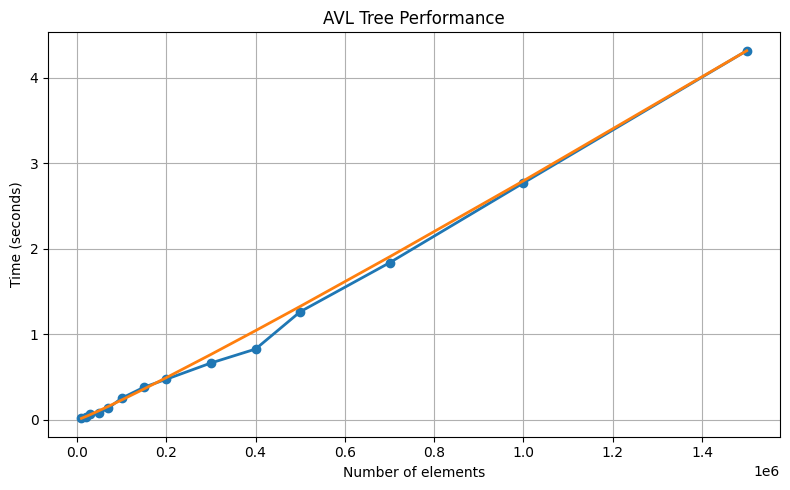
\includegraphics[width=0.9\textwidth]{avl_nlogn_overlay.png}
	\caption{Сравнение экспериментального времени работы программы с теоретической зависимостью $n \log n$.}
\end{figure}

Анализ графика показывает, что экспериментальная зависимость времени выполнения близка к функции $n \log n$. При увеличении объёма входных данных наблюдается рост времени, превышающий линейный, что объясняется логарифмической составляющей сложности операций в сбалансированном дереве.

Поскольку каждая операция (вставка, поиск, удаление) в AVL-дереве выполняется за $O(\log n)$, суммарное время выполнения последовательности из $n$ операций имеет сложность $O(n \log n)$.

Таким образом, экспериментальные результаты согласуются с теоретической оценкой сложности алгоритмов, реализованных в программе.

\subsection*{Недочёты}

В ходе разработки программы были выявлены некоторые ограничения и потенциальные недостатки реализации.

Во-первых, при работе с памятью используется динамическое выделение памяти (оператор new) без явной обработки исключений. В случае нехватки памяти программа может завершиться аварийно, так как обработка ошибки выделения памяти не реализована.

Во-вторых, реализация операций сохранения и загрузки словаря предполагает корректность формата входного файла. Несмотря на наличие базовых проверок, при повреждении файла возможны ситуации, когда загрузка завершается неуспешно без детальной диагностики причины ошибки.

Также стоит отметить, что в реализации используется рекурсивный подход для операций вставки, удаления и обхода дерева. При теоретически возможной глубине рекурсии это может привести к переполнению стека, однако в сбалансированном AVL-дереве такая ситуация маловероятна.

Кроме того, сравнение строк выполняется посимвольно, что может оказывать влияние на производительность при работе с длинными ключами (до 256 символов), однако в рамках поставленной задачи это не является критичным.

В целом программа корректно реализует требуемую функциональность и проходит тесты, однако указанные особенности могут быть учтены при дальнейшем улучшении реализации.

\subsection*{Выводы}

В ходе выполнения лабораторной работы была реализована структура данных «словарь» на основе AVL-дерева, обеспечивающая эффективное хранение и обработку пар «ключ–значение».

Данная структура может применяться в задачах, где требуется поддерживать упорядоченные данные с быстрым поиском, вставкой и удалением элементов. К типовым областям применения относятся:
\begin{itemize}
	\item реализация словарей и ассоциативных массивов;
	\item обработка текстовых данных (поиск слов, подсчёт частот);
	\item хранение и обработка индексированных данных;
	\item системы, требующие гарантированного времени выполнения операций.
\end{itemize}

Все основные операции (поиск, вставка, удаление) в AVL-дереве выполняются за $O(\log n)$, что обеспечивается за счёт поддержания сбалансированности дерева. Экспериментальные результаты показали, что суммарное время выполнения последовательности операций соответствует оценке $O(n \log n)$. По памяти реализованная структура данных имеет сложность $O(n)$, так как для хранения каждого элемента словаря создаётся отдельный узел дерева. Каждый узел содержит ключ фиксированного максимального размера, значение, а также указатели на дочерние элементы и вспомогательные данные (высоту поддерева).

Реализация данной структуры данных требует аккуратного подхода, так как необходимо корректно поддерживать высоту узлов и выполнять балансировку дерева при вставке и удалении элементов. Наибольшую сложность представляет реализация операции удаления, связанная с перестроением структуры дерева и сохранением его свойств.

В процессе разработки были решены задачи корректной балансировки дерева, обработки строковых ключей и организации эффективного хранения данных. Полученная программа успешно проходит тестирование и соответствует поставленным требованиям. 

\end{document}

